\section{Accuracy for OpenML-CC18 Tasks}
\label{app:cc18}

\begin{figure}[!htpb]
\centering

\includegraphics[width=0.8\columnwidth]{figures/cc18_wide}
  \caption{Classifications on the OpenML-CC18 datasets with max sample size, number of features, and number of classes. The 100-tree classifiers include: Extremely Simple Streaming Forest \textbf{(XForest-100T)}, Mondrian Forest \textbf{(MF-100T)}, Random Forest \textbf{(RF-100T)} and Gradient Boosting \textbf{(GB-100T)}. 
  All plots show averaged accuracy over five folds and are listed in the order of dataset IDs. Sample sizes correspond to respective datasets. In many tasks, XForests exceed MFs and perform as well as, sometimes even better than, RFs and GBs. Moreover, XForest accuracy consistently increases with new samples across different data domains.
  }
\label{fig:cc18}
\end{figure}

\clearpage

\section{Wall Times for Three Selected Tasks}
\label{app:select_time}

\begin{figure*}[!htb]
\centering
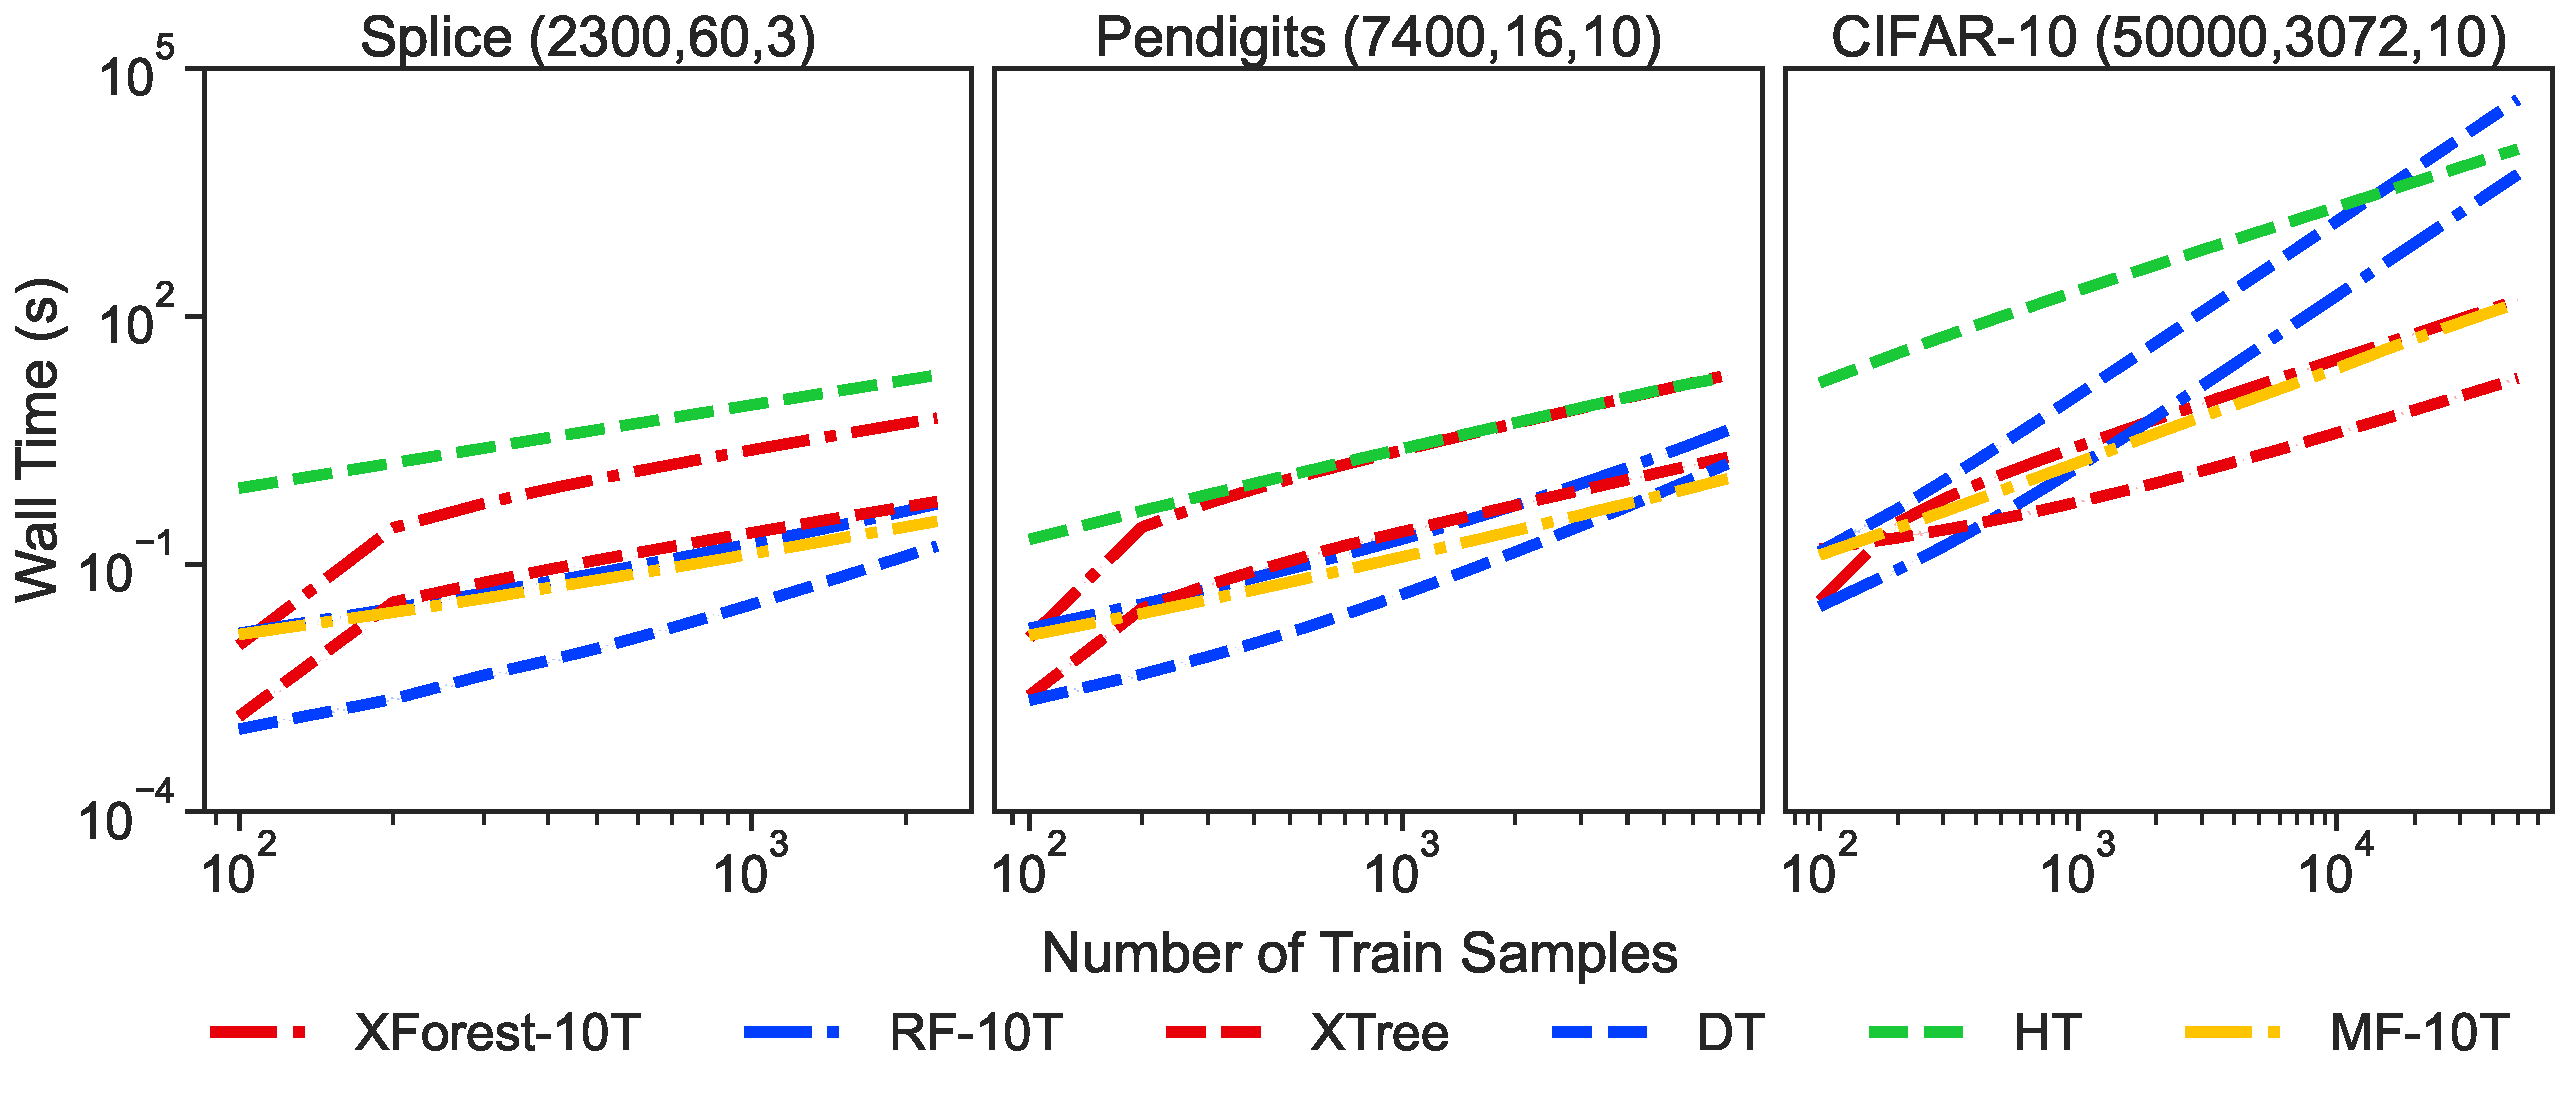
\includegraphics[width=0.9\textwidth]{figures/select_time}
  \caption{Training wall times on the Splice \textbf{(left)}, Pendigits \textbf{(center)}, and CIFAR-10 \textbf{(right)} datasets. The panel titles include the maximum sample size, the number of features, and the number of classes.
  The classifiers include: Extremely Simple Streaming Forest with 10 trees \textbf{(XForest-10T)}, Random Forest with 10 trees \textbf{(RF-10T)}, Extremely Simple Streaming Tree \textbf{(XTree)}, Decision Tree \textbf{(DT)}, Hoeffding Tree \textbf{(HT)}, and Mondrian Forest with 10 trees \textbf{(MF-10T)}. 
  Each line represents averaged results from \textbf{10 randomized repetitions}.
  Cumulative fitting times are shown for all estimators, and two batch estimators' times include refitting at each sample size. XTrees are the most efficient in the CIFAR-10 task. XForests take longer times in the Splice and Pendigits tasks, but are overtaken by HTs, batch DTs, and RFs in the CIFAR-10 task. MFs maintain similar time efficiency as XForests. RFs are faster than DTs in the CIFAR-10 task, which could be attributed to the feature reductions.
  }
\label{fig:select_time}
\end{figure*}

In terms of training wall times, XTrees are the most efficient on the CIFAR-10 dataset (Figure \ref{fig:select_time}, right). 
XForests take longer times in the Splice and Pendigits tasks (Figure \ref{fig:select_time}, left and center). However, on the CIFAR-10 dataset, HTs are the most inefficient streaming trees, even slower than the two streaming ensembles. Also, as sample size increases, time usage of batch estimators grows more quickly due to refitting, and they surpass XForests around 2,000 samples. MFs take similar training times as XForests.
% , which could be attributed to a limited number of estimators (only 10 trees)
All training wall times grow linearly as sample size increases. Results are subject to implementation details of packages used (Section \ref{methods}).

\clearpage

\section{XOR and XNOR Tasks}
\label{app:xor_xnor}

\begin{figure*}[!htb]
\centering
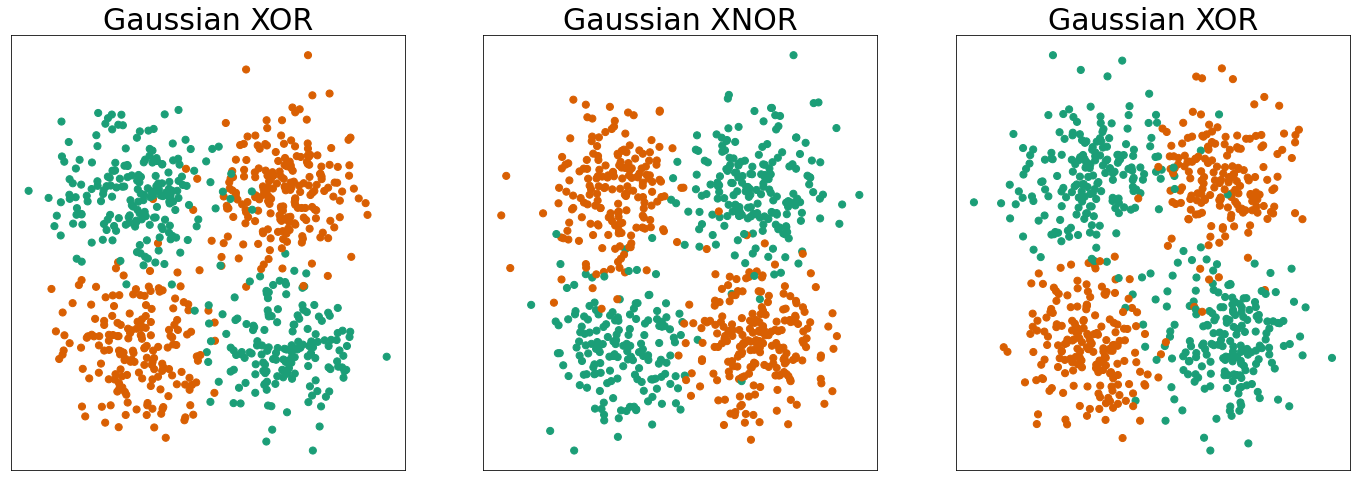
\includegraphics[width=0.9\textwidth]{figures/gaussian_xor_xnor}

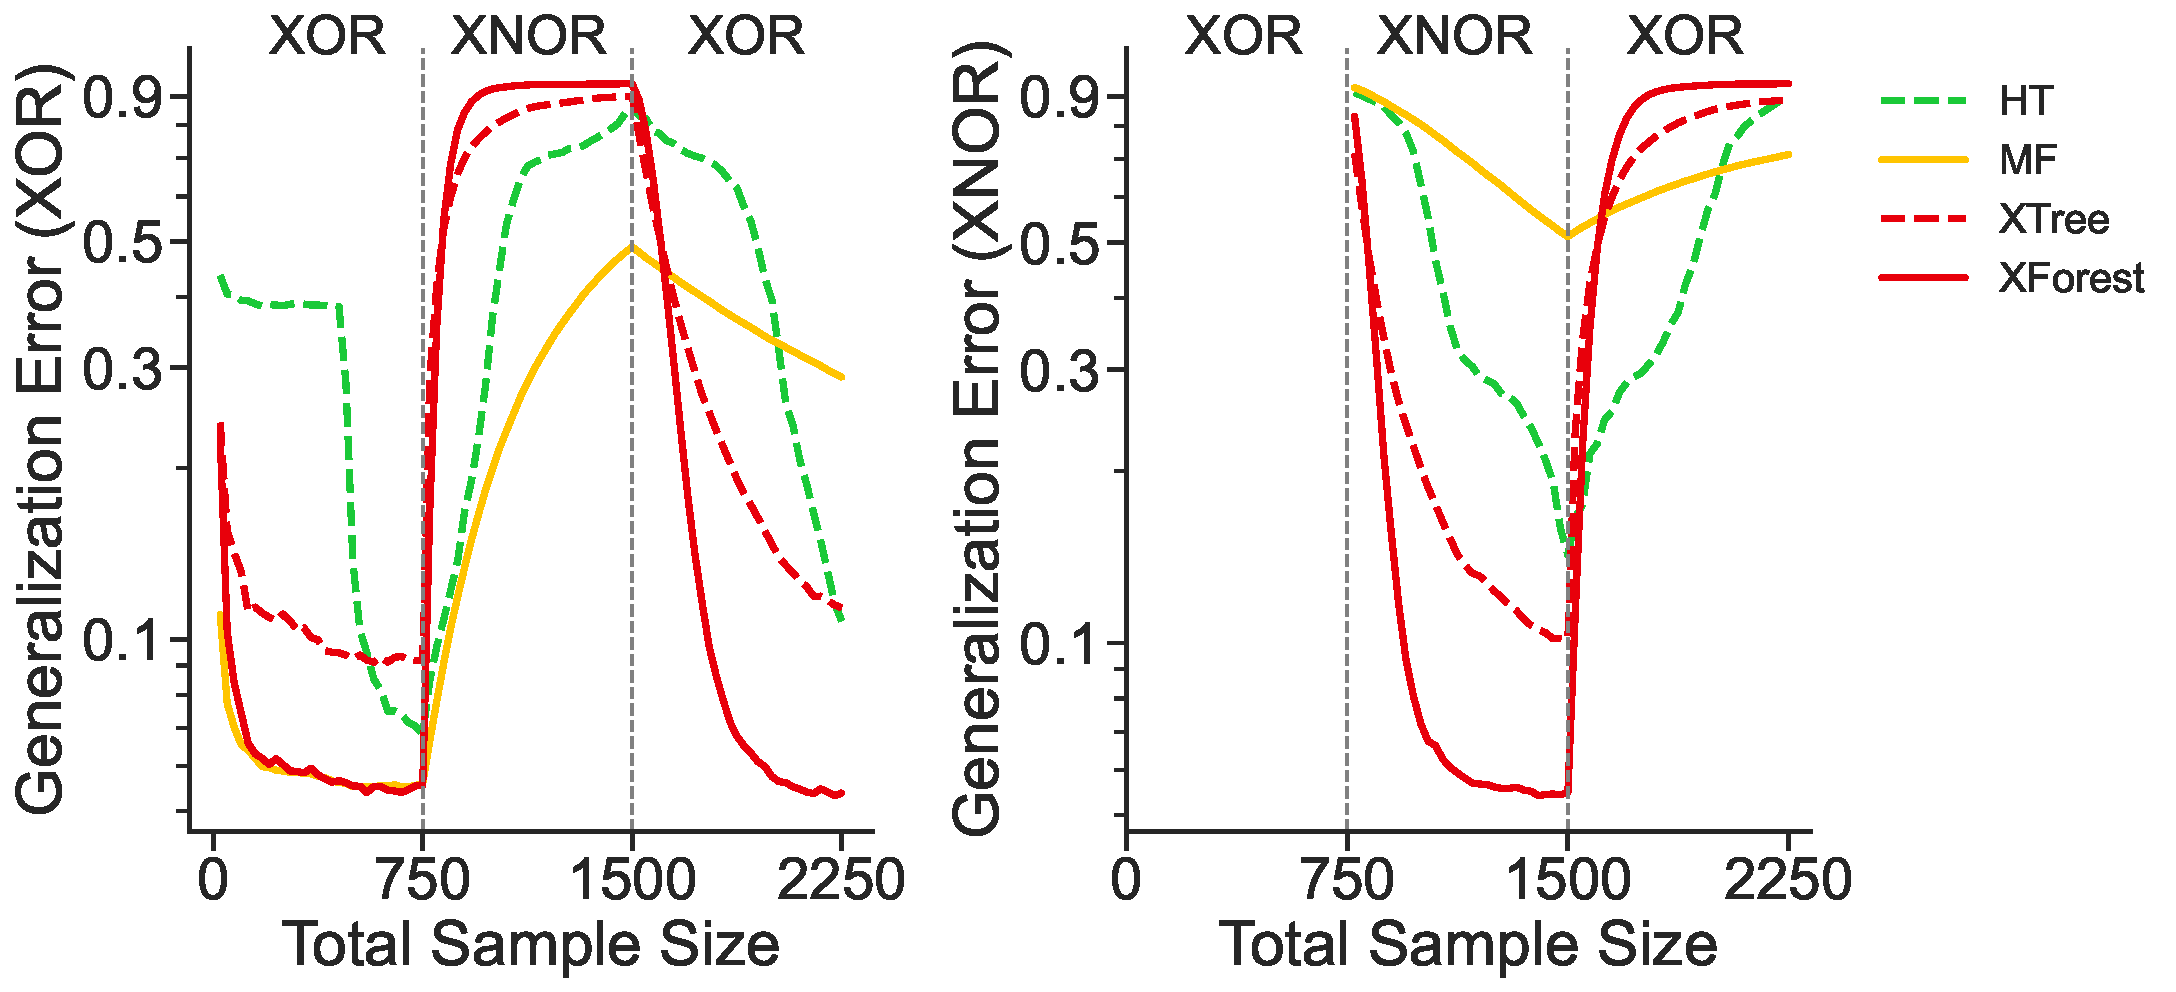
\includegraphics[width=0.9\textwidth]{figures/xor_xnor}
  \caption{Distribution shift adaptation with Gaussian XOR and XNOR. XForests and XTrees adapt quickly to the new distribution after both shifts. 
  }
\label{fig:xor_xnor}
\end{figure*}

Figure \ref{fig:xor_xnor} shows XForests and XTrees can adapt to two distribution shifts in data batches. Top row shows 3 subsets of 750 samples belonging to two types of distributions. Gaussian XNOR has the same distribution as Gaussian XOR but with the inverse class labels. Data are introduced in batches of 25 samples at a time, and the distribution shifts at 750 samples and 1,500 samples. HTs have slower adaptation, while MFs fail to achieve good performance after both shifts.

\clearpage

\section{XOR and R-XOR Tasks}
\label{app:xor_rxor}


\begin{figure*}[!htb]
\centering
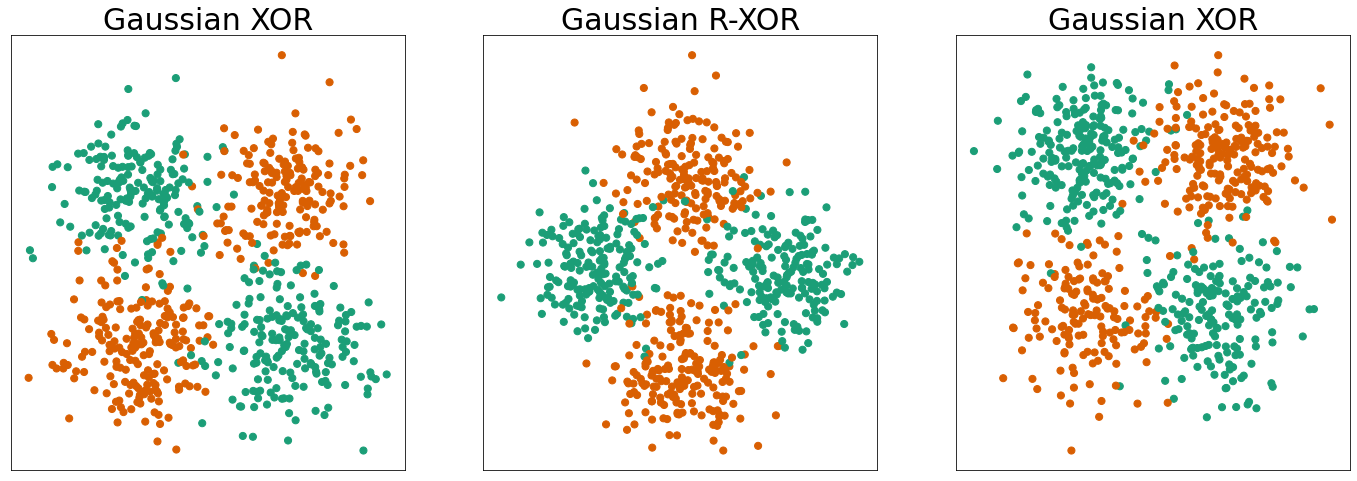
\includegraphics[width=0.9\textwidth]{figures/gaussian_xor_rxor}
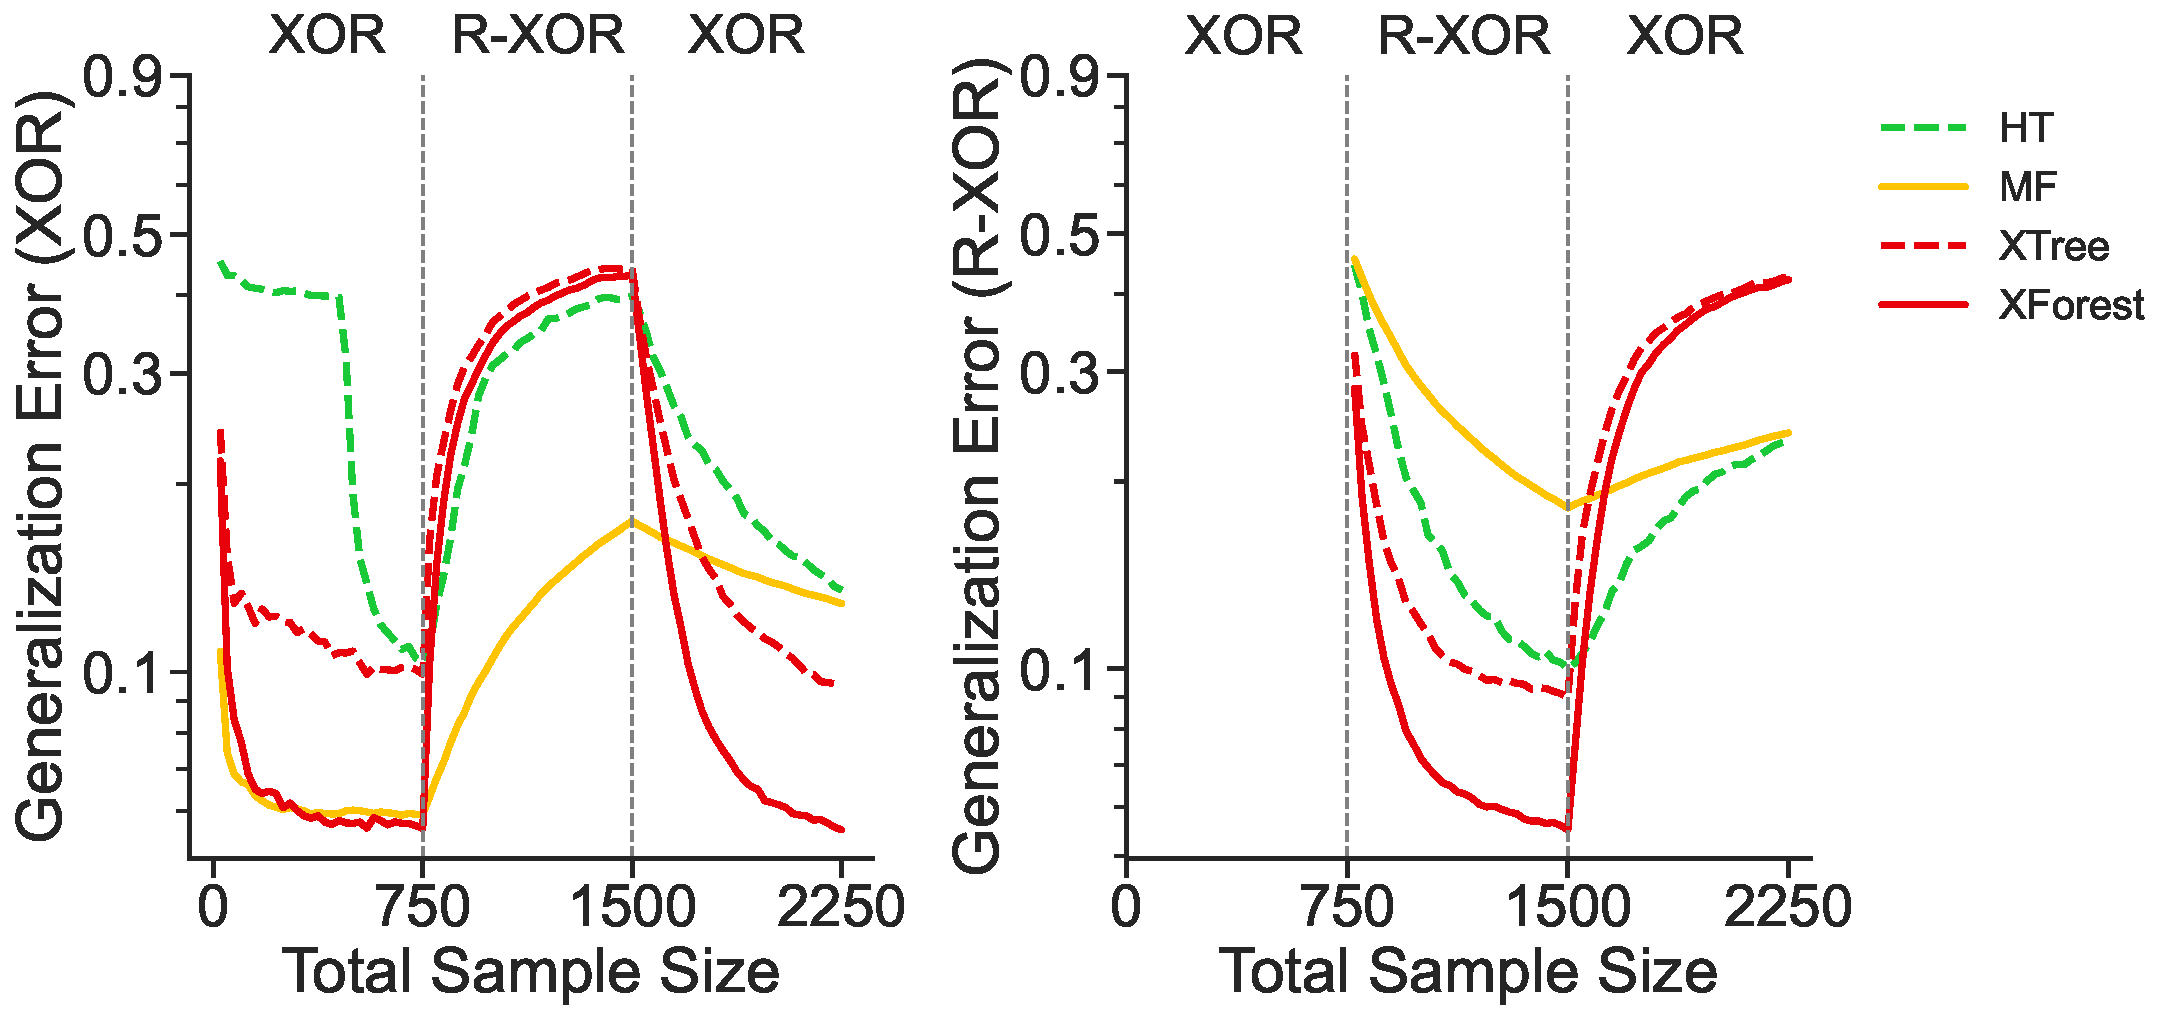
\includegraphics[width=0.9\textwidth]{figures/xor_rxor}
  \caption{Distribution shift adaptation with Gaussian XOR and R-XOR. XForests and XTrees adapt quickly to the new distribution after both shifts. 
  }
\label{fig:xor_rxor}
\end{figure*}

Figure \ref{fig:xor_rxor} shows XForests and XTrees can adapt to two distribution shifts in data batches. Top row shows 3 subsets of 750 samples belonging to two types of distributions. Gaussian R-XOR has the same distribution as Gaussian XOR but with the class labels rotated 45 degrees. Data are introduced in batches of 25 samples at a time, and the distribution shifts at 750 samples and 1,500 samples. HTs have slower adaptation, while MFs fail to achieve good performance after both shifts.